\section{Exterior Helmholtz problems}
\label{Sec2:exteriorHelmholtz}
Scattering problems involve \textit{unbounded exterior domains}, $\Omega^+$. A common method for solving such problems with the FEM is to introduce an artificial boundary that encloses the scatterer. On the artificial boundary some sort of absorbing boundary condition (ABC) is prescribed. The problem is then reduced to a finite domain, and both the elastic scatterer and the bounded domain between the scatterer and the artificial boundary can be discretized with finite elements. Several methods exist for handling the exterior Helmholtz problem (on unbounded domain), including
\begin{itemize}
	\item the perfectly matched layer (PML) method after B{\'e}renger~\cite{Berenger1994apm,Berenger1996pml}
	\item the boundary element method~\cite{Sauter2011bem,Schanz2007bea,Marburg2008cao,Chandler_Wilde2012nab}
	\item Dirichlet to Neumann-operators (DtN-operators)~\cite{Givoli2013nmf}
	\item local differential ABC operators~\cite{Shirron1995soe,Bayliss1982bcf,Hagstrom1998afo,Tezaur2001tdf}
	\item the infinite element method.~\cite{Bettess1977ie,Bettess1977dar}
\end{itemize}
Herein, the infinite element method is chosen. For the IEM, the unbounded domain $\Omega^+$ is partitioned into two domains by the artificial boundary $\Gamma_{\mathrm{a}}$; $\Omega_{\mathrm{a}}$ and $\Omega_{\mathrm{a}}^+$ (see \Cref{Fig2:artificialBoundary}). 
\begin{figure}
	\centering
	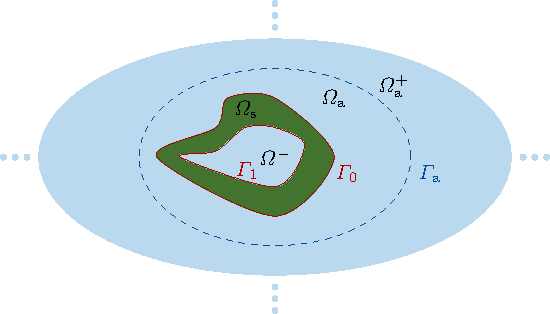
\includegraphics[scale=1]{../../LaTeX/createFigures/TikzFigures/articleIGA_PhD/artificialBoundary}
%	\includegraphics[scale=1]{\graphicsFolder/Figure3}
	\caption[Illustration of artificial boundary]{An artificial boundary $\Gamma_{\mathrm{a}}$ is introduced such that the exterior domain $\Omega^+$ is decomposed by the two domains $\Omega_{\mathrm{a}}$ (which is bounded by $\Gamma_0$ and $\Gamma_{\mathrm{a}}$) and $\Omega_{\mathrm{a}}^+$. Thus, $\Omega^+ = \Omega_{\mathrm{a}} \cup \Omega_{\mathrm{a}}^+$.}
	\label{Fig2:artificialBoundary}
\end{figure}
These domains are discretized by finite and infinite elements, respectively. A convergence analysis of a coupled FEM-IEM can be found in \cite{Demkowicz2001aoa}.

The exterior Helmholtz problem is given by
\begin{alignat}{3}
	\nabla^2 p + k^2 p &= 0 	&&\text{in}\quad \Omega^+,\label{Eq2:HelmholtzEqn}\\
	\partial_n p &= g						&&\text{on}\quad \Gamma_0,\label{Eq2:HelmholtzEqnNeumannCond}\\
	\pderiv{p}{r}-\imag k p &= o\left(r^{-1}\right)\quad &&\text{with}\quad r=|\vec{x}|\label{Eq2:sommerfeldCond}
\end{alignat}
where the Sommerfeld condition~\cite{Sommerfeld1949pde} in \Cref{Eq2:sommerfeldCond} restricts the field in the limit $r\to\infty$ uniformly in $\hat{\vec{x}}=\frac{\vec{x}}{r}$, such that no waves originate from infinity. The Neumann condition given by the function $g$ will in the case of rigid scattering be given by the incident wave $p_{\mathrm{inc}}$. Zero displacement of the fluid normal on the scatterer (rigid scattering) implies that $\partial_n(p+p_{\mathrm{inc}}) = 0$ where $\partial_n$ denotes the partial derivative in the normal direction on the surface $\Gamma_0$ (pointing ``out'' from $\Omega^+$), which implies that
\begin{equation}
	g = -\pderiv{p_{\mathrm{inc}}}{n}.
\end{equation}
Plane incident waves (with amplitude $P_{\mathrm{inc}}$) traveling in the direction $\vec{d}_{\mathrm{s}}$ can be written as
\begin{equation}\label{Eq2:p_inc}
	p_{\mathrm{inc}} = P_{\mathrm{inc}}\euler^{\imag k\vec{d}_{\mathrm{s}}\cdot\vec{x}}.
\end{equation}
The normal derivative on the surface of any smooth geometry may then be computed by
\begin{align}
	\pderiv{p_{\mathrm{inc}}}{n} &= \vec{n}\cdot\nabla p_{\mathrm{inc}} = \imag k\vec{d}_{\mathrm{s}}\cdot\vec{n} p_{\mathrm{inc}}.
\end{align}

\subsection{Weak formulation for the Helmholtz equation}
In order to choose the correct solution space in the infinite element method, the asymptotic behavior of the scattered pressure $p$ at large radii\footnote{Here, $r$ is referred to as the radius even though it does not necessarily represent the radius in spherical coordinates.} $r$ must be examined. In~\cite{Wilcox1956aet}, Wilcox shows that the scalar pressure field $p(\vec{x})$ satisfying the Helmholtz equation and the Sommerfeld radiation conditions can be written in the form\footnote{In some appropriate coordinate system $(r,\vartheta,\varphi)$ with the ``radial variable'', $r$, extending to infinity. Typically, some degeneration of the ellipsoidal (in 3D) coordinate system.}
\begin{equation}\label{Eq2:wilcoxExpansion}
	p(\vec{x}) = \frac{\euler^{\imag kr}}{r}\sum_{n=0}^\infty \frac{p_n(\vartheta,\varphi)}{r^n},
\end{equation}
which implies that $|p|=\bigoh(r^{-1})$ asymptotically for large $r$. Considering a function which represents this asymptotic property
\begin{equation}
	\Psi(r)=\frac{\euler^{\imag kr}}{r},
\end{equation}
one can observe that the $L^2$ Hermitian inner product does not exist. Indeed, if $\Gamma_0$ is the unit sphere then
\begin{equation*}
	(\Psi,\Psi)_{L^2} = \int_{\Omega^+} \frac{\euler^{\imag kr}}{r}\frac{\euler^{-\imag kr}}{r} \idiff \Omega= 4\PI\int_1^\infty \frac{1}{r^2}r^2\idiff r,
\end{equation*}
which is not finite. The solution to the problem is to introduce weighted norms by defining the inner product
\begin{equation}
	(p,q)_w = \int_{\Omega^+} wp\bar{q}\idiff\Omega,\qquad\text{with}\quad w= \frac{1}{r^2}.
\end{equation}
The following norm may then be induced
\begin{equation}
	\| p\|_{1,w} = \sqrt{(p,p)_w + (\nabla p,\nabla p)_w}
\end{equation}
such that the trial functions satisfy $\| p\|_{1,w}<\infty$. The integrals
\begin{equation}
	\int_{\Omega^+} p\bar{q}\idiff\Omega\quad\text{and}\quad\int_{\Omega^+}\nabla p\cdot\nabla\bar{q}\idiff\Omega
\end{equation}
are well defined if the test functions $q$ are such that
\begin{equation}
	(q,q)_{w^*}<\infty\quad\text{and}\quad (\nabla q,\nabla q)_{w^*}<\infty
\end{equation}
with the inner product
\begin{equation}
	(p,q)_{w^*} = \int_{\Omega^+} w^*p\bar{q}\idiff\Omega,\qquad\text{with}\quad w^*= r^2,
\end{equation}
and the corresponding norm
\begin{equation}
	\| p\|_{1,w^*} = \sqrt{(p,p)_{w^*} + (\nabla p,\nabla p)_{w^*}}.
\end{equation}
Define now the following \textit{weighted Sobolev spaces} for the trial- and test spaces
\begin{equation}
	H_w^1(\Omega^+) = \{p\,:\,\| p\|_{1,w} < \infty\}\quad\text{and}\quad H_{w^*}^1(\Omega^+) =  \{q\,:\,\| q\|_{1,w^*} < \infty\},
\end{equation}
respectively. These definitions will not ensure that all trial function satisfy the Sommerfeld condition. Leis solved this problem in~\cite{Leis1986ibv} by modifying the trial space to be
\begin{equation}
	H_w^{1+}(\Omega^+) = \{p\,:\,\| p\|_{1,w}^+ < \infty\}
\end{equation}
where
\begin{equation}
	\| p\|_{1,w}^+ = \sqrt{\| p\|_{1,w}^2 + \int_{\Omega^+}\left|\pderiv{p}{r} - \imag kp\right|^2\idiff\Omega}.
\end{equation}
For a more detailed discussion of the functional analysis involved in these spaces refer to the book by Ihlenburg~\cite[pp. 41-43]{Ihlenburg1998fea}.

The weak form of the Helmholtz equation may now be found by multiplying \Cref{Eq2:HelmholtzEqn} with a test function and integration over the domain
\begin{equation*}
	\int_{\Omega^+} \left[q\nabla^2 p + k^2 qp\right]\idiff \Omega = 0.
\end{equation*}
Using Greens first identity this can be written as
\begin{equation*}
	-\int_{\Omega^+} \nabla q\cdot\nabla p\idiff\Omega + \int_{\partial\Omega^+} q\nabla p\cdot\vec{n}\idiff\Gamma + k^2\int_{\Omega^+}  qp\idiff \Omega = 0.
\end{equation*}
Thus,
\begin{equation}\label{Eq2:weakformulationHelmholtz}
	\int_{\Omega^+} \nabla q\cdot\nabla p\idiff\Omega -  k^2\int_{\Omega^+}qp\idiff\Omega = \int_{\partial\Omega^+} q g\idiff\Gamma.
\end{equation}
The weak formulation then becomes: 
\begin{equation}
	\text{Find} \quad p\in H_w^{1+}(\Omega^+)\quad\text{such that}\quad B(q,p) = L(q),\qquad \forall q\in H_{w^*}^1(\Omega^+),
\end{equation}
where the bilinear form is given by
\begin{equation*}
	B(q,p) = \int_{\Omega^+} \left[\nabla q\cdot\nabla p-  k^2qp\right]\idiff\Omega
\end{equation*}
and the corresponding linear form is given by
\begin{equation*}
	L(q) = \int_{\Gamma_0} qg\idiff\Gamma.
\end{equation*}


\subsection{Infinite elements}
\label{se:infElems}
In the following, a derivation of the weak formulation for infinite elements using a prolate spheroidal coordinate system is presented (cf.~\cite{Burnett1994atd}). The IEM is typically presented with four infinite element formulations:
\begin{itemize}
	\item Petrov--Galerkin conjugated (PGC)
	\item Petrov--Galerkin unconjugated (PGU)
	\item Bubnov--Galerkin conjugated (BGC)
	\item Bubnov--Galerkin unconjugated (BGU)
\end{itemize}
The Petrov--Galerkin formulations are based on the weighted Sobolev spaces after Leis~\cite{Leis1986ibv}. It turns out that it is possible to create Bubnov--Galerkin formulations as well when the integration in the weak formulation is understood in the sense of the Cauchy principal value (consider~\cite{Burnett1994atd} and~\cite{Gerdes1998tcv} for details). These spaces differ compared to the Petrov--Galerkin counterpart in that the test space and trial space are equal. The difference between the conjugated formulations and the unconjugated formulations is simply conjugations of the test functions in the weak formulation. The accuracy of these formulations has been assessed in the overview in~\cite{Astley2000ief}.

The idea of the IEM is to partition the unbounded domain $\Omega^+$ into $\Omega_{\mathrm{a}}$ and $\Omega_{\mathrm{a}}^+$ separated by an artificial boundary $\Gamma_{\mathrm{a}}$ (cf. \Cref{Fig2:artificialBoundary}). These two domains can then be discretized with finite elements and infinite elements, respectively. The boundary of the scatterer is assumed to be parameterized using 3D NURBS surface patches, such that the domain $\Omega_{\mathrm{a}}$ can be parameterized using 3D NURBS volume patches. Denote by $\calV_h(\Omega_{\mathrm{a}})$, the space spanned by these trivariate NURBS-basis functions. As the 3D NURBS volume representation of $\Omega_{\mathrm{a}}$ reduces to a NURBS surface parametrization at $\Gamma_{\mathrm{a}}$, a natural partition of $\Gamma_{\mathrm{a}}$ into surface elements arises. Denote by $\calV_h(\Gamma_{\mathrm{a}})$, the space spanned by the resulting bivariate basis functions. Consider now the following basis of the \textit{radial shape functions} which is motivated by the Wilcox expansion in \Cref{Eq2:wilcoxExpansion}
\begin{equation}
	\calI_{N, w}^+ = \mathrm{span}\left(\left\{\frac{\euler^{\imag k r}}{r^n}\right\}_{n=1,\dots,N}\right).
\end{equation}
Moreover, define corresponding spaces for the test-space
\begin{equation}
\calI_{N, w^*}^+ = \begin{cases}
	\calI_{N, w}^+  & \text{ for Bubnov--Galerkin formulations}\\
	\mathrm{span}\left(\left\{\frac{\euler^{\imag k r}}{r^{n+2}}\right\}_{n=1,\dots,N}\right) & \text{ for Petrov--Galerkin formulations}.
	\end{cases}
\end{equation}
The trial- and test spaces for the infinite elements can then be defined by
\begin{align}
	\calI_{h, w}^+ &= \calV_h(\Gamma_{\mathrm{a}})\times \calI_{N, w}^+,\\
	\calI_{h, w^*}^+ &= \calV_h(\Gamma_{\mathrm{a}})\times \calI_{N, w^*}^+,
\end{align}
respectively. Finally, the trial- and test spaces for the coupled FEM-IEM can be written as
\begin{align}
	\calF^+_{h,w} &= \left\{p\in H_w^{1+}(\Omega^+);\, p\big|_{\Omega_{\mathrm{a}}}\in \calV_h(\Omega_{\mathrm{a}})\quad\text{and}\quad p\big|_{\Omega_{\mathrm{a}}^+}\in \calI_{h, w}^+\right\},\\
	\calF^+_{h,w^*} &= \left\{q\in H_{w^*}^{1+}(\Omega^+);\, q\big|_{\Omega_{\mathrm{a}}}\in \calV_h(\Omega_{\mathrm{a}})\quad\text{and}\quad q\big|_{\Omega_{\mathrm{a}}^+}\in \calI_{h, w^*}^+\right\},
\end{align}
respectively. Note that $\calF^+_{h,w^*}=\calF^+_{h,w}$ for Bubnov--Galerkin formulations.

For the unconjugated formulations the Galerkin formulations now takes the form: 
\begin{equation}\label{Eq2:GalerkinFormulationHelmholtz}
	\text{Find}\quad p_h\in \calF^+_{h,w}\quad \text{such that} \quad B_{\mathrm{uc}}(q_h, p_h) = L(q_h),\qquad \forall q_h\in \calF^+_{h,w^*}
\end{equation}
where the bilinear form and linear form are respectively given by
\begin{align}\label{Eq2:infElemntBilinearForm}
	B_{\mathrm{uc}}(q,p) &= \lim_{\gamma\to\infty}\left(\int_{\Omega^\gamma} \left[\nabla q\cdot \nabla p - k^2 qp\right]\idiff\Omega - \int_{S^\gamma} q\partial_n p\idiff\Gamma\right),\\
	L(q) &= \int_{\Gamma_0} qg\idiff\Gamma.\nonumber
\end{align}
Here, $S^\gamma$ is the surface at $r = \gamma$ (and $\Omega^\gamma$ is the domain bounded by $\Gamma_0$ and $S^\gamma$, such that $\lim_{\gamma\to\infty}\Omega^\gamma = \Omega^+$) and the full domain can then be recovered by letting $\gamma\to\infty$ (see \Cref{Fig2:model3_in_waterInf}). Recall that $\partial_n p = \frac{\partial p}{\partial n}= \vec{n}\cdot\nabla p$ where $\vec{n}$ is pointing ``out'' of $\Omega^\gamma$. In the conjugated formulations the test functions $q_h$ are conjugated.

Let $r_{\mathrm{a}}$ be the radius in the prolate spheroidal coordinate system at the artificial boundary $\Gamma_{\mathrm{a}}$. Moreover, let the radial shape functions $\phi$ be defined by
\begin{equation}
	\phi_m(r) = \euler^{\imag k (r-r_{\mathrm{a}})}Q_m\left(\frac{r_{\mathrm{a}}}{r}\right),\quad m = 1,\dots,N
\end{equation}
where 
\begin{equation}\label{Eq2:Q_m}
	Q_m(x) = \sum_{\tilde{m}=1}^N D_{m\tilde{m}} x^{\tilde{m}}
\end{equation}
is a set of polynomial functions defined on the half open interval $(0,1]$. To obtain optimal sparsity of the global matrix, one should choose the polynomials such that $Q_m(1) = \delta_{m1}$, with the Kronecker delta function defined by
\begin{equation}\label{Eq2:Kronecker}
	\delta_{ij} = \begin{cases}
		1 & \text{if}\quad i = j\\
		0 & \text{if}\quad i \neq j
		\end{cases}
\end{equation}
which implies that $\phi_m(r_{\mathrm{a}}) = \delta_{m1}$. In~\cite{Burnett1994atd} Burnett includes the restrictions $\phi_m(r_n) = \delta_{mn}$ with radii $r_n$, $n=1,\dots,N$ (see \Cref{Fig2:model3_in_waterInf}).
\begin{figure}
	\centering
	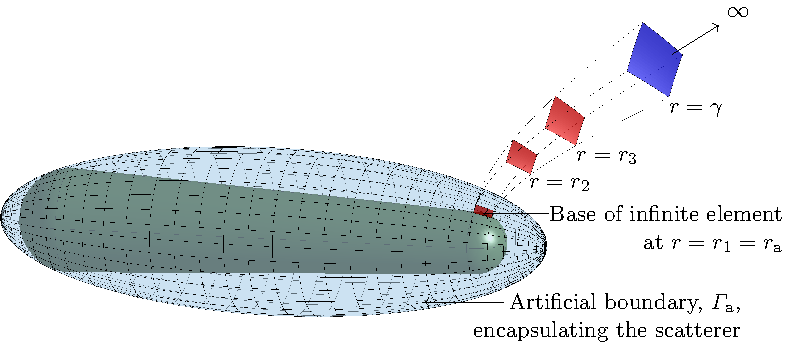
\includegraphics[scale=1]{../../LaTeX/createFigures/TikzFigures/articleIGA_PhD/model3_inWaterInf}
%	\includegraphics[scale=1]{\graphicsFolder/Figure4}
	\caption{Illustration of an infinite element (with $N=3$) where the radial shape functions have the Kronecker delta property at radii $r_1=r_{\mathrm{a}}$, $r_2=\frac54 r_{\mathrm{a}}$ and ${r_3=\frac64 r_{\mathrm{a}}}$. The (green) scatterer inside $\Gamma_{\mathrm{a}}$ is the BeTSSi submarine which originates from the BeTSSi workshops~\cite{Gilroy2013bib}. Note that the volume elements discretizing the domain $\Omega_{\mathrm{a}}$ (bounded by the scatterer and the artificial boundary) are not shown here.}
	\label{Fig2:model3_in_waterInf}
\end{figure} 
Alternatively, one could use the shifted Chebyshev polynomials as done by Shirron and Dey in~\cite{Shirron2002aie}. These polynomials are defined by the three-term recurrence relation
\begin{equation}
	\tilde{T}_{m+1}(x) = 2(2x-1)\tilde{T}_m(x) - \tilde{T}_{m-1}(x)
\end{equation}
for $m\geq 1$ starting with
\begin{equation}
	\tilde{T}_0(x) = 1\quad\text{and}\quad\tilde{T}_1(x) = 2x-1.
\end{equation}
Let
\begin{equation}
	Q_m(x) = \begin{cases}x\left(\tilde{T}_{m-1}(x)-1\right)& m>1\\
				x & m=1.
				\end{cases}
\end{equation}
Then the coefficients $D_{m\tilde{m}}$ in \Cref{Eq2:Q_m} can be collected in the matrix (for $N \leq 6$)
\begin{equation*}
	\vec{D} = \begin{bmatrix}
		1 & 0 & 0 & 0 & 0 & 0\\
		-2 & 2 & 0 & 0 & 0 & 0\\	
		0 & -8 & 8 & 0 & 0 & 0\\
		-2 & 18 & -48 & 32 & 0 & 0\\
		0 & -32 & 160 & -256 & 128 & 0\\
		-2 & 50 & -400 & 1120 & -1280 & 512
	\end{bmatrix}.
\end{equation*}
For the Petrov--Galerkin formulations, a second set of shape functions (for the test space) must be created, namely
\begin{equation}
	\psi_n(r) = \euler^{\imag k (r-r_{\mathrm{a}})}\tilde{Q}_n\left(\frac{r_{\mathrm{a}}}{r}\right),\quad n = 1,\dots,N
\end{equation}
using
\begin{equation}
	\tilde{Q}_n(x) = \sum_{\tilde{n}=1}^N \tilde{D}_{n\tilde{n}} x^{\tilde{n}+2}
\end{equation}
where it is natural to choose $\tilde{D}_{n\tilde{n}}=D_{n\tilde{n}}$. The Bubnov--Galerkin formulations use the same shape functions for the test space, i.e., $\psi_n = \phi_n$.

Alternatively, the polynomials $Q$ can be based upon the Bernstein basis of order $\check{p}=N-1$ by
\begin{equation}
	Q_m(x) = xb_{p-m+1,\check{p}}(x)\qquad m=1,\dots N
\end{equation}
where
\begin{equation}
	b_{i,\check{p}}(x) = \binom{n}{i}(1-x)^{\check{p}-i}x^i = \sum_{j=0}^{\check{p}-i}(-1)^j\binom{\check{p}}{i}\binom{\check{p}-i}{j} x^{i+j},\qquad i=0,\dots,\check{p}.
\end{equation}

For completeness, note that the coefficients for the radial shape functions used by Burnett~\cite{Burnett1994atd} (for the Bubnov--Galerkin formulations) can be found by solving $\vec{D}\vec{B} = \vec{E}$ where
\begin{equation*}
	\vec{B} = \begin{bmatrix}
		x_1 & x_2 & \dots & x_N\\
		x_1^2 & x_2^2 & \dots & x_N^2\\
		\vdots & \vdots & \ddots & \vdots\\
		x_1^N & x_2^N & \dots & x_N^N\\
	\end{bmatrix},\quad \vec{E} = \begin{bmatrix}
		1 	& 	&  & \\
		   	& \euler^{\imag k (r_{\mathrm{a}}-r_2)} & & \\
			&  		& \ddots 	&\\
			&  		& 			& \euler^{\imag k (r_{\mathrm{a}}-r_N)}
	\end{bmatrix}, \quad x_n = \frac{r_{\mathrm{a}}}{r_n}.
\end{equation*}
The coefficients $D_{m\tilde{m}}$ are thus given by $\vec{D} = \vec{E}\vec{B}^{-1}$. For Petrov--Galerkin formulations, the coefficients $\tilde{D}_{n\tilde{n}}$ are found in the same way, but now with the matrix
\begin{equation*}
	\tilde{\vec{B}} = \begin{bmatrix}
		x_1^3 & x_2^3 & \dots & x_N^3\\
		x_1^4 & x_2^4 & \dots & x_N^4\\
		\vdots & \vdots & \ddots & \vdots\\
		x_1^{N+2} & x_2^{N+2} & \dots & x_N^{N+2}\\
	\end{bmatrix}
\end{equation*}
instead of $\vec{B}$. So, with the notation presented, these basis functions are based on the Lagrange polynomials with polynomial order\footnote{The usage of a check sign above the polynomial order $p$ is to avoid ambiguity between the polynomial order and the scattered pressure.} $\check{p}=N-1$
\begin{equation}
	l_n(x) = \prod_{\substack{0\leq n\leq \check{p}\\ n\neq m}} \frac{x-x_n}{x_m-x_n},
\end{equation}
since the polynomials $Q_m$ can be written as
\begin{equation*}
	Q_m(x) = \euler^{\imag k(r_{\mathrm{a}}-r_m)} \frac{r_m}{r_{\mathrm{a}}} xl_m(x)
\end{equation*}
such that
\begin{equation*}
	\phi_m(r) = \euler^{\imag k(r-r_m)}\frac{r_m}{r}l_m\left(\frac{r_{\mathrm{a}}}{r}\right).
\end{equation*}
The radial shape functions in the test space for the Petrov--Galerkin formulations take the form
\begin{equation*}
	\psi_n(r) = \euler^{\imag k(r-r_n)}\left(\frac{r_n}{r}\right)^3 l_n\left(\frac{r_{\mathrm{a}}}{r}\right).
\end{equation*}
As all these sets of basis functions span the same space, they should only affect the conditioning of the system. Note that the sets of basis functions are identical for $N=1$.

The trial- and test functions now take the form 
\begin{equation}\label{Eq2:p_h}
	p_h(\vec{x}) = \begin{dcases}
		\sum_{J\in\vec{\kappa}_{\mathrm{a}}} \sum_{m=1}^N d_{m,J}\phi_m(r) R_J(\xi,\eta,\zeta)\big|_{\Gamma_{\mathrm{a}}} & \vec{x}\in\Omega_{\mathrm{a}}^+\\
		\sum_{J\in\vec{\kappa}} d_{1,J} R_J(\xi,\eta,\zeta) & \vec{x}\in\Omega_{\mathrm{a}}
	\end{dcases}
\end{equation}
and
\begin{equation}\label{Eq2:q_h}
	q_h(\vec{x}) = \begin{dcases}
		\sum_{I\in\vec{\kappa}_{\mathrm{a}}} \sum_{n=1}^N c_{n,I}\psi_n(r) R_I(\xi,\eta,\zeta)\big|_{\Gamma_{\mathrm{a}}} & \vec{x}\in\Omega_{\mathrm{a}}^+\\
		\sum_{I\in\vec{\kappa}} c_{1,I} R_I(\xi,\eta,\zeta) & \vec{x}\in\Omega_{\mathrm{a}},
	\end{dcases}
\end{equation}
respectively. Here, $\vec{\kappa}$ is the collection of the global indices of the NURBS basis functions and $\vec{\kappa}_{\mathrm{a}}$ the corresponding indices of the non-zero NURBS function at the surface $\Gamma_{\mathrm{a}}$. Moreover, $R_I(\xi,\eta,\zeta)$ is the set of NURBS basis functions. The system of equations will now be obtained by inserting the functions in \Cref{Eq2:p_h} and \Cref{Eq2:q_h} into the bilinear form (or sesquilinear form for the BGC and PGC formulations, i.e. the bilinear form with conjugated test functions). 

Before the insertion, it is advantageous to split the bilinear form in \Cref{Eq2:infElemntBilinearForm} as
\begin{equation}\label{Eq2:SplittingOfB_uc}
	B_{\mathrm{uc}}(q,p) = B_{\mathrm{a}}(q,p) + B_{\mathrm{uc},\mathrm{a}}^+(q,p)
\end{equation}
where
\begin{align}
	B_{\mathrm{a}}(q,p) &= \int_{\Omega_{\mathrm{a}}} \left[\nabla q\cdot \nabla p - k^2 qp\right]\idiff\Omega\nonumber\\
	B_{\mathrm{uc},\mathrm{a}}^+(q,p) &= \lim_{\gamma\to\infty}\left(\int_{\Omega_{\mathrm{a}}^\gamma} \left[\nabla q\cdot \nabla p - k^2 qp\right]\idiff\Omega - \int_{S^\gamma} q\partial_n p\idiff\Gamma\right).\label{Eq2:B_uc_a}	
\end{align}
Insertion of \Cref{Eq2:p_h} and \Cref{Eq2:q_h} into \Cref{Eq2:GalerkinFormulationHelmholtz} (using the splitting in \Cref{Eq2:SplittingOfB_uc}) results in the following system of equations
\begin{equation}
	(\vec{A}_{\mathrm{a}} + \vec{A}_{\mathrm{uc},\mathrm{a}}^+)\vec{d} = \vec{F}
\end{equation}
with components
\begin{alignat*}{3}
	& &&\vec{A}_{\mathrm{a}}[I,J] = B_{\mathrm{a}}(R_I,R_J)\qquad I, && J = 1,\dots,|\boldsymbol\kappa|\\
	& &&\vec{F}[I] = L(R_I)\qquad && I = 1,\dots,|\boldsymbol\kappa|\\
	& &&\vec{d}[J] = d_{1,J}\qquad && J = 1,\dots,|\boldsymbol\kappa|
\end{alignat*}
and
\begin{align*}
	\vec{A}_{\mathrm{uc},\mathrm{a}}^+[\tilde{I},\tilde{J}] &= B_{\mathrm{uc},\mathrm{a}}^+(R_I\psi_n,R_J\phi_m)\\
	\vec{d}[\tilde{J}] &= d_{m,J}
\end{align*}
where $I = \boldsymbol\kappa_{\mathrm{a}}[\tilde{i}]$ and $J = \boldsymbol\kappa_{\mathrm{a}}[\tilde{j}]$ for $\tilde{i},\tilde{j}=1,\dots,|\boldsymbol\kappa_{\mathrm{a}}|$ and $m,n=1,\dots,N$, and
\begin{align*}
	\tilde{I} &= \begin{cases}\boldsymbol\kappa_{\mathrm{a}}[\tilde{i}] & n = 1\\
	|\boldsymbol\kappa|+(n-2)|\boldsymbol\kappa_{\mathrm{a}}|+\tilde{i} & n>1\end{cases}\\
	\tilde{J} &= \begin{cases}\boldsymbol\kappa_{\mathrm{a}}[\tilde{j}] & m = 1\\
	|\boldsymbol\kappa|+(m-2)|\boldsymbol\kappa_{\mathrm{a}}|+\tilde{j} & m>1.\end{cases}
\end{align*}
Note that $\vec{A}_{\mathrm{a}}$ and $\vec{F}$ are independent of the IEM and that there are $|\boldsymbol\kappa| +|\boldsymbol\kappa_{\mathrm{a}}|(N-1)$ linear equations. The matrices are assembled as in the classical FEM. That is, instead of looping through the indices, one loops through the elements. A formula for $B_{\mathrm{uc},\mathrm{a}}^+(R_I\psi_n,R_J\phi_m)$ for the Petrov Galerkin formulation is derived in \Cref{Sec2:AppendixDerivationOfBilinearForm} and the final bilinear form is given in \Cref{Eq2:finalBilinearFormB_uc_a}. The final formulas for the other three formulations are also added in this appendix.

\subsection{Far field pattern}
The problem is solved inside an artificial boundary, computing the so-called near field. However, the far field is also often of interest. To solve this issue, one uses the integral solution given by\footnote{For the conjugated formulations one may also compute the far field using the radial shape functions in the infinite elements, but for the unconjugated formulations it is mentioned in~\cite[p. 137]{Shirron1998aco} that the expansion does not converge in the far field, such that it must be computed by other means.} (cf.~\cite[Theorem 2.21]{Chandler_Wilde2012nab})
\begin{equation}\label{Eq2:KirchhoffIntegral}
	p(\vec{x}) = \int_{\Gamma_0}\left[ p(\vec{y})\pderiv{\Phi_k(\vec{x},\vec{y})}{n(\vec{y})} - \Phi_k(\vec{x},\vec{y})\pderiv{p(\vec{y})}{n(\vec{y})}\right]\idiff \Gamma(\vec{y})
\end{equation}
where $\vec{y}$ is a point on the surface $\Gamma_0$, $n$ lies on $\Gamma_0$ pointing ``into'' $\Omega^+$ at $\vec{y}$ and $\Phi_k$ is the free space Green's function for the Helmholtz equation in \Cref{Eq2:HelmholtzEqn} given (in 3D) by
\begin{equation}\label{Eq2:FreeSpaceGrensFunction}
	\Phi_k(\vec{x},\vec{y}) = \frac{\euler^{\imag kR}}{4\PI R},\quad\text{where}\quad R = |\vec{x} - \vec{y}|.
\end{equation}
The derivative of both Green's function and the numerical solution for the pressure is therefore needed
\begin{equation}
	\pderiv{\Phi_k(\vec{x},\vec{y})}{n(\vec{y})} = \frac{\Phi_k(\vec{x},\vec{y})}{R}(\imag kR-1)\pderiv{R}{n(\vec{y})},\quad\text{where}\quad\pderiv{R}{n(\vec{y})} = -\frac{(\vec{x}-\vec{y})\cdot\vec{n}(\vec{y})}{R}.
\end{equation}
Note that for sound-hard scattering (where $\partial_n(p+p_{\mathrm{inc}}) = 0$) the values for $\partial_n p$ are known at the boundary $\Gamma_0$ (given by \Cref{Eq2:HelmholtzEqnNeumannCond}). To use the exact expression for the derivative seems to give better results and is for this reason used in the sound-hard scattering cases when computing the field outside the artificial boundary.

The \textit{far field pattern} for the scattered pressure $p$, is now defined by
\begin{equation}\label{Eq2:farfield}
	p_0(\hat{\vec{x}}) =  \lim_{r\to\infty} r \euler^{-\imag k r}p(r\hat{\vec{x}}),
\end{equation}
with $r = |\vec{x}|$ and $\hat{\vec{x}} = \vec{x}/|\vec{x}|$. Using the limits
\begin{equation}\label{Eq2:Phi_k_limits1}
	\lim_{r\to\infty} r\euler^{-\imag k r}\Phi_k(r\hat{\vec{x}},\vec{y}) = \frac{1}{4\PI}\euler^{-\imag k \hat{\vec{x}}\cdot\vec{y}}
\end{equation}
and
\begin{equation} \label{Eq2:Phi_k_limits2}
	\lim_{r\to\infty} r\euler^{-\imag k r}\pderiv{\Phi_k(r\hat{\vec{x}},\vec{y})}{n(\vec{y})} = -\frac{\imag k}{4\PI}\euler^{-\imag k \hat{\vec{x}}\cdot\vec{y}}\hat{\vec{x}}\cdot\vec{n}(\vec{y})
\end{equation}
the formula in \Cref{Eq2:KirchhoffIntegral} simplifies in the far field to (cf.~\cite[p. 32]{Ihlenburg1998fea})
\begin{equation}\label{Eq2:KirchhoffIntegralFarField}
	p_0(\hat{\vec{x}}) = -\frac{1}{4\PI}\int_{\Gamma_0}\left[ \imag k p(\vec{y})\hat{\vec{x}}\cdot\vec{n}(\vec{y}) + \pderiv{p(\vec{y})}{n(\vec{y})}\right]\euler^{-\imag k \hat{\vec{x}}\cdot\vec{y}}\idiff \Gamma(\vec{y}).
\end{equation}
From the far field pattern, the \textit{target strength}, $\TS$, can be computed. It is defined by
\begin{equation}\label{Eq2:TS}
	\TS = 20\log_{10}\left(\frac{|p_0(\hat{\vec{x}})|}{|P_{\mathrm{inc}}|}\right)
\end{equation}
where $P_{\mathrm{inc}}$ is the amplitude of the incident wave at the geometric center of the scatterer (i.e. the origin). Note that $\TS$ is independent of $P_{\mathrm{inc}}$, which is a result of the linear dependency of the amplitude of the incident wave in scattering problems (i.e. doubling the amplitude of the incident wave will double the amplitude of the scattered wave).